\section{Mixed Reality}
\label{sec-2}
\fbox{
\parbox{\linewidth}{
	\textit{Ziel des Kapitels:}\\
	Begriffsklärung und Einordnung von AR,MR,VR in das Virtual Continuum. Einordnung der HoloLens in das gegebene Spektrum. Bildet wichtige Grundlage für die zu entwickelnden Konzepte. Davon ausgehend kurz Potential für Anwendungen aufzeigen.\\[6px]
	\textit{Inhalte:}	
	\begin{itemize}
		\item Virtual Continuum erklären und AR, AV, VR einordnen
		\item (Je nach Relevanz) Dazu kurz Techniken und Devices erwähnen: HMDs, Smartphones, Lighthouse Tracking, Inside-Out Tracking, Gemeinsamer Nullpunkt, Object Tracking, Object Recognition…
		\item Potential für MR und HoloLens aufzeigen
	\end{itemize}
	
	\textit{Wichtige Literatur:}	
	\begin{itemize}
		\item A taxonomy of mixed reality visual displays \cite{Milgram94}
		\item A survey of augmented reality \cite{Azuma97}
		\item Augmented Reality: Where we will all live \cite{Peddie17}
	\end{itemize}
}}

\subsection{Das Virtual Continuum}
\label{sec-2-1}
Virtual Continuum vorstellen und Begriffe AR; AV; VR; MR klären und einordnen.

\begin{figure}[h!]
	\centering
	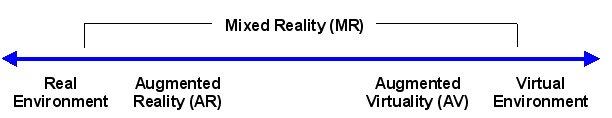
\includegraphics[width=0.9\textwidth]{images/virtual_continuum.png}
	\caption{Virtual Continuum eingeführt von Paul Milgram \cite{Milgram94}}
	\label{img:virtual_continuum}
\end{figure}

\subsection{AR und VR Devices}

HoloLens einordnen und kurz andere Techniken erwähnen, damit unterschiedliche Arbeiten in Kapitel 4 entsprechend eingeordnet werden können. Smartphone AR, z.B. Apple ARKit, Pokemon Go, HUDs, Oculus Rift, Vive, PS VR, Opaque vs see through, standalone vs wired, Bezug zu anderen Techniken ansprechen: Object detection, Object recognition, Object tracking

\subsection{Beispiele Anwendungen}
HoloMuse, Galaxy Explorer, Fragments, LifeLiqe, HoloTour, Insight Heart, Dynamic Anatomy\\
Damit Orientierungshilfe gegeben und Vorstellungsvermögen verbessert für späteres Anwendungsdesign

\subsection{Aktuelle Entwicklung und Potential für MR}
Leistungssteigerung im Hardwarebereich und Fortschritte bei AI führt zur Verfügbarkeit von Devices von AR bis VR, daher sehr aktuelles Thema, viel Potential



